\documentclass[crop, tikz]{standalone}
\usepackage{tikz}

\usetikzlibrary{positioning, decorations.pathmorphing}
\begin{document}

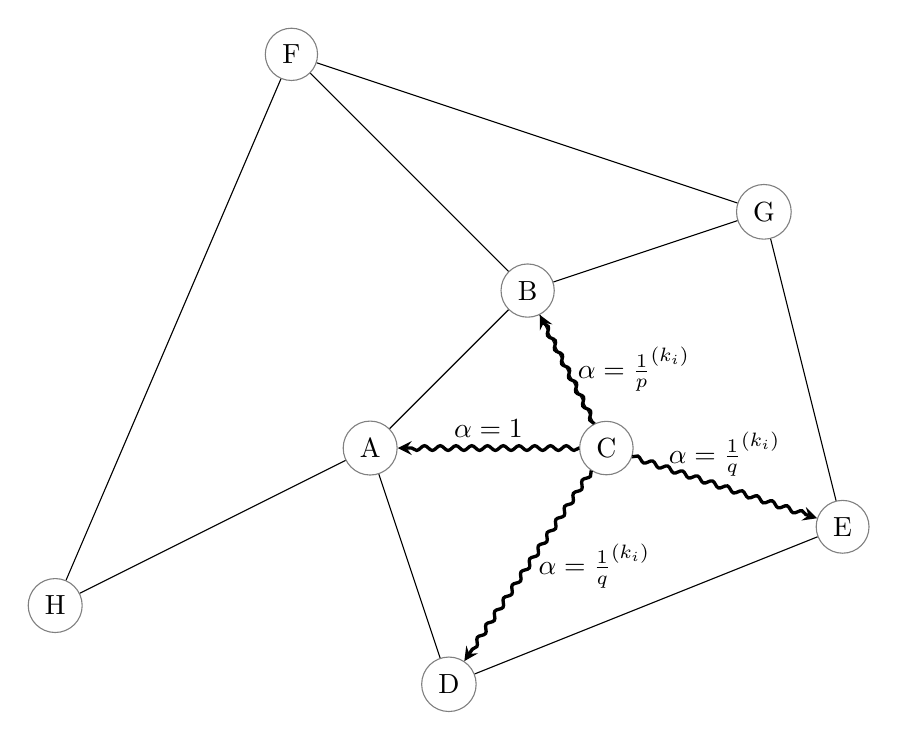
\begin{tikzpicture}
    \node[shape=circle, draw=gray] (A) at (0, 0) {A};
    \node[shape=circle, draw=gray] (B) at (2, 2) {B};
    \node[shape=circle, draw=gray] (C) at (3, 0) {C};
    \node[shape=circle, draw=gray] (D) at (1, -3) {D};
    \node[shape=circle, draw=gray] (E) at (6, -1) {E};
    \node[shape=circle, draw=gray] (F) at (-1, 5) {F};
    \node[shape=circle, draw=gray] (G) at (5, 3) {G};
    \node[shape=circle, draw=gray] (H) at (-4, -2) {H};
    

    \path [-] (F) edge node[left] {} (B);
    \path [-] (H) edge node[left] {} (F);
    \path [-] (A) edge node[left] {} (H);
    \path [-] (A) edge node[left] {} (D);
    \path [-] (G) edge node[left] {} (F);
    \path [-] (C) edge node[left] {} (B);
    \path [-] (A) edge node[left] {} (B);
    \path [-] (B) edge node[left] {} (G);
    \path [-] (G) edge node[left] {} (E);
    
    \path [-] (E) edge node[left] {} (D);
    

    \draw[-stealth, very thick, decoration={snake, pre length=0.01mm, segment length=2mm, amplitude=0.3mm, post length=1.0mm}, decorate,] (C) -- node[midway, above] {$\alpha={1}$} (A);
     \draw[-stealth, very thick, decoration={snake, pre length=0.01mm, segment length=2mm, amplitude=0.3mm, post length=1.0mm}, decorate,] (C) -- node[midway, above] {$\alpha={\frac{1}{q}}^{(k_i)}$} (E);
      \draw[-stealth, very thick, decoration={snake, pre length=0.01mm, segment length=2mm, amplitude=0.3mm, post length=1.0mm}, decorate,] (C) -- node[right] {$\alpha={\frac{1}{q}}^{(k_i)}$} (D);
       \draw[-stealth, very thick, decoration={snake, pre length=0.01mm, segment length=2mm, amplitude=0.3mm, post length=1.0mm}, decorate,] (C) -- node[right] {$\alpha={\frac{1}{p}}^{(k_i)}$} (B);
\end{tikzpicture}

\end{document}

